\subsection{Research Cycles}
\label{subsec:research-cycles}

Following the three-cycle framework formalized by \citeonline{hevner_2004} and \citeonline{hevner_2007}, this research operates across three interdependent cycles---the \textit{Relevance Cycle} (connecting the research to the operational cloud-native environment and problem context), the \textit{Rigor Cycle} (grounding the design in foundational kernel theories and prior scientific literature), and the central \textit{Design Cycle} (iteratively building and evaluating the artifact)---as depicted in Figure~\ref{fig:dsr-cycles}.

\begin{figure}[ht]
    \centering
    \caption{Design Science Research Cycles}
    \label{fig:dsr-cycles}
    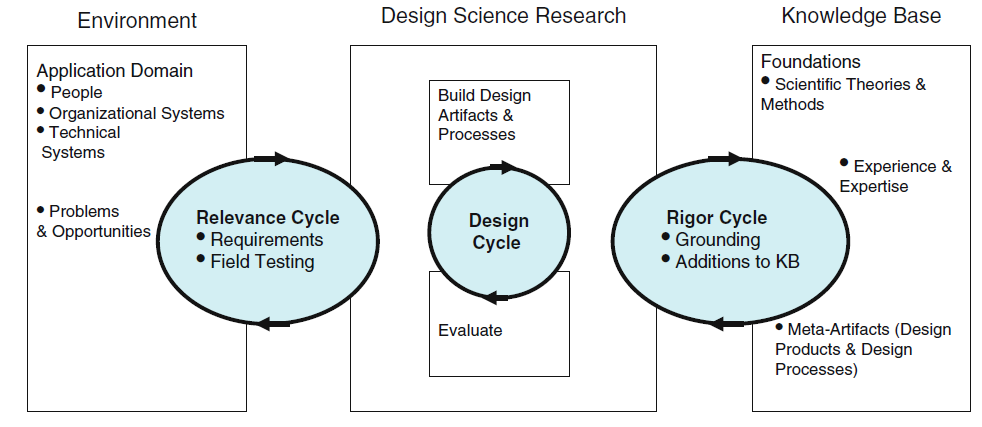
\includegraphics[width=1.0\linewidth]{images/methodology/hevner-dsr-cycles.png}
    \par\medskip\ABNTEXfontereduzida\selectfont\textbf{Source:} \cite{hevner_2004} \par\medskip
\end{figure}
